\documentclass[12pt, final]{article}
\usepackage{fullpage,amsthm,amsfonts,amsmath}
\usepackage{enumerate}
\usepackage[margin=1in]{geometry}
\usepackage{color}
\usepackage{epsfig}
\usepackage{epstopdf}
\usepackage{datatool}
\usepackage{array}
\usepackage{tabu}
\usepackage{amsmath}
\usepackage{caption}
\usepackage{float}
\usepackage{tabularx, booktabs}
\usepackage{pdfpages}
\usepackage{standalone}
\usepackage{hyperref}
\usepackage{subfigure}
\usepackage{graphicx}
\hypersetup{colorlinks = true, urlcolor = blue, filecolor = blue, linkcolor = blue}
\floatstyle{plaintop}
\restylefloat{table}
\renewcommand{\thefootnote}{$\star$} 
\begin{document}
\title{Team 40: Predicting Mortality in ICU Setting (Project Draft).}

\date{\today}

%%
\renewcommand{\thefootnote}{$\dag$}
%%
\author{Vincent La\footnote{vincent.la@gatech.edu}, Avi Ananthakrishnan\footnote{avinash.ananthakrishnan@gatech.edu}}

\maketitle

\begin{abstract}
Medical data capturing and electronic health records are now improving to the point where we are rapidly improving the amount and quality of data we get about a patient. Socioeconomic data is often captured such as race, marital status, and even insurance type (e.g. Medicaid or Medicare). Electronic Health Record (EHR) systems often track key clinical values like certain labs, prescription history, and acute diagnoses. We also have access to real-time vital signs that becomes available in intensive care unit (ICU) settings. However, the challenge comes in modeling this data due to the high density and heterogeneous data types. Furthermore, because any modeling will ultimately support human decision making (doctors and other clinical staff), interpretability comes at a premium. Because of this, using natural language processing tools to decompose free-text clinical notes into meaningful features is very attractive and valuable since it offers a potentially richer set of meaningful features that are hard to capture in structured form. In this project, we fit three models: a baseline model composing purely of static and demographic features, a model with structured clinical data (e.g. labs, diagnoses, prescriptions), and a model that uses the same features as the previous two but is augmented using topics extracted from conducting Latent Dirichlet Allocation (LDA) on charts and notes data associated with the patient. The baseline model achieves an AUROC of about 70\%. The improved models are still a work in progress and we will report on their progress in the final draft. We also want to thank Dr. Kumar Dharmarajan, a geriatrician, who helped provide some clinical context on the top few topics that LDA abstracted.
\end{abstract} 

\newpage
%%%%%
\renewcommand{\thefootnote}{\number\value{footnote}} 
%%%%%
\section{Introduction} \label{Introduction}
Accurate knowledge of patient's clinical state is critical in a clinical setting. Patients in an intensive care unit are particularly in a critical state. Thus, if we can have better accurate mortality prediction within an ICU, we can use this to better understand which patients should be prioritized for clinical care and how we can better allocate resources. Within an ICU, there are many measurements being made from from various devices, but we know that there are both problems in terms of false positives and false negatives. While false negatives might seem to be more problematic, being too sensitive and introducing a lot of false positives also has problems as well. Too many false positives results in information fatigue and providers lose trust in signal as it's hard to separate from noise. By improving mortality prediction using data from EMRs and other clinically-relevant data, we can provide better predictions to improve efficiency and quality of care.

\section{Background and Literature Review}
\label{Background and Lit Review}
Siontis et. al (2011) \cite{Siontis} provide an empirical review of methodologies around mortality models. In this paper, the authors use Medline to identify studies published in 2009 that assessed AUC of predicting all cause mortality. What they find is that most studies at the time predicted mortality with modest accuracy, with large variability across populations, which makes sense since for since very high risk populations it may be easier to predict mortality, but for lower risk general populations, the class imbalance is very high with relatively few patients actually dying.
\\
\\
We note that there have been many attempts to predict mortality, with some models being quite complicated. However, there have also been more technically simple models that attempt to predict mortality. For example, in DeSalvo et. al (2005) \cite{DeSalvo}, the authors attempt to predict mortality using a single question: ``In general, would you say your health is ... Excellent, Very Good, Good, Fair, or Poor". Similarly, we will provide a baseline model that only uses demographics and static variables (see Table \ref{Features} for the specific variables used) as features to predict mortality. While we know that we can do better using a richer feature set, doing a simple model with demographics and static variables provides us with a baseline to benchmark against.
\\
\\
Next, there are a few papers that actually use the MIMIC III data for mortality prediction using ICU data. In Unfolding Physiological State: Mortality Model in Intensive Care Units, Ghassemi et. al (2014)\cite{Ghassemi}, the authors use Latent Variables Models to decompose free-text hospital notes into meaningful features to predict patient mortality. For the actual prediction, they use linear SVM in various setting (e.g. patient first arrives at hospital, In hospital mortality, 30 day mortality, etc.) and they largely find that using hospital notes improved AUCs.

\section{Methodology}
\label{Methodology}

As in Ghassemi et. al (2014) \cite{Ghassemi}, we will ultimately use free-text hospital notes predict mortality following an admission to the hospital. We believe that using features extracted from free-text will improve on existing mortality models since it will provide more nuanced topics that add additional signal to structured data (e.g. labs, diagnoses, prescriptions).
\\
\\
We use the MIMIC III data set. We will then perform topic modeling, using Latent Dirichlet Allocation (LDA), to do natural language processing on the notes to extract meaningful topics. In terms of evaluating our model, we will predict mortality following the admission. For example, to evaluate 24 hour mortality predictions, in the training set, we will create a 24 hour prediction window and using the data that is transformed into features, we will measure AUC of mortality where outcome variable is mortality within 24 hours. We will then test on held-out test data set to report final test AUC.

\subsection{Data Exploration}
\label{Data Exploration}
The dataset contains 58,976 distinct hospital admissions with 46,520 distinct patients. Thus, most people in this dataset were admitted once, but there is also a long tail of readmissions. About 39,000 patients were admitted once, with 5,160 admitted twice. However, there s a long tail of about 2,000 remaining patients who have been admitted more than twice in this time period, with the maximum being 42 admissions over this time period. Furthermore, we note that admission lengths on average are about 10 days, but the median length of stay is closer to 6.5 days. This makes sense as again, the distribution is likely right skewed.
\\
\\
Next, we look at the breakdown of admissions by patients' insurance. This is interesting because the type of insurance a patient has is likely to be very correlated with patient characteristics. For example, Medicare patients will likely be older and have more acute risk. Medicaid is likely correlated with meaningful socioeconomic characteristics. As expected, many of the patients are Medicare patients, at about 48\% of the total population. This makes sense as Medicare patients are older and higher risk, so will comprise more of the admissions.

\begin{figure}[H]
\centering
\caption{Admissions Deaths}
\label{AdmissionsDeaths}
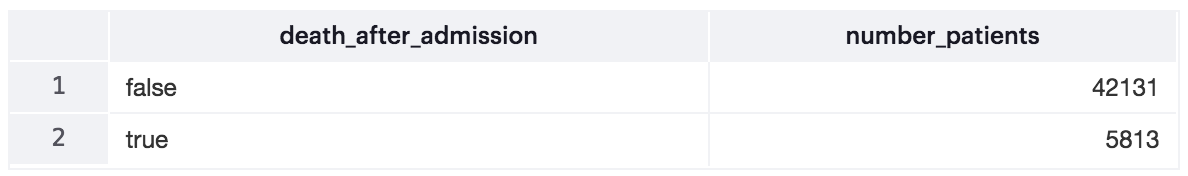
\includegraphics[page = {1}, scale = 0.4]{./images/admissions-deaths.png}
\end{figure}

In addition, we note that about 5,800 patients are recorded as having died at some point after the admission. 

\subsection{Feature Extraction}
Now that we have done some data exploration, this next section will discuss feature extraction and what features we actually used in our model to predict mortality.

\begin{table}[H]
\footnotesize
\newcolumntype{C}{>{\centering\arraybackslash}X}% centering
\caption{Features}
\label{Features}
\centering
\begin{tabularx}{\textwidth}{l C C}\hline
 & (1) & (2) \\\
Categories & Features & Extracted \\ \hline
 &  &   \\
Demographic and Static Features & Age, Gender, Ethnicity, Admission Type, Insurance Type &  \\\
\\\
Vital Signs & Heart Rate & Min, Max \\\
\\\
Clinical Notes & Topics using LDA &  \\\
\end{tabularx}
\end{table}

\subsubsection{Topic Modeling: LDA}
To extract additional features, we conduct LDA on Note Events table within MIMIC III. We first tokenize the dataset by splitting the text into sentences and sentences into words. We lowercase all words and remove punctuation. Words fewer than 3 characters are removed. We use the $gensim$ and $nltk$ libraries and remove all stop words from $gensim$. We create a TF-IDF (Term Frequency - Inverse Document Frequency) model object and run LDA using TF-IDF to create topics. Examples of the topics created are shown below.

\begin{table}[H]
\footnotesize
\newcolumntype{C}{>{\centering\arraybackslash}X}% centering
\caption{Examples of Topics Returned by LDA}
\label{LDA}
\centering
\begin{tabularx}{\textwidth}{l C C}\hline
 & (1) \\\
Topic Number & Top Words \\ \hline
 &    \\\
0 & contrast, mass, head, imag, brain  \\\
1 & effus, pleural, lung, chang, portabl \\\
2 & spine, arteri, carotid, imag, cervic
\end{tabularx}
\end{table}

\subsection{Model Architecture}
\label{Model Architecture}

\subsubsection{Baseline Model}
We first provide a baseline model that is a Random Forest model that only uses the Demographic and Static Features as described in Table \ref{Features}. The purpose of this is to provide a simple model that can serve as a baseline. We then split the data into 70\% Training and 30\% Test, so the Training dataset had 41,283 rows and the Test data set contained 17,693 rows. We then use Stratified K-Fold Validation with $n_splits = 6$. For features, we one-hot encoded $admission_type$, $insurance$, $language$, $marital_status$, and $ethnicity$. In the end, this yielded a total of 137 features, one for each value, including when the value is null.

\subsubsection{Improved Model: With Structured Clinical Data}
We will then create an improved model above baseline that uses all the same features but also adds structured clinical data such as labs, prescriptions, and previous utilization. We will use a similar Training/Test split.

\subsubsection{Best Model: Using LDA}
Our last model will use the same features as in the previous models, but will also include features for each topic returned by LDA on charts relevant to the admission for each patient.

\section{Experimental Results}
\label{Experimental Results}

\subsubsection{Baseline Model}
We first show results of the baseline Random Forest model that only uses the Demographic and Static Features as described in Table \ref{Features}.

\begin{figure}[H]
\centering     %%% not \center
\subfigure[ROC]{\label{fig:a}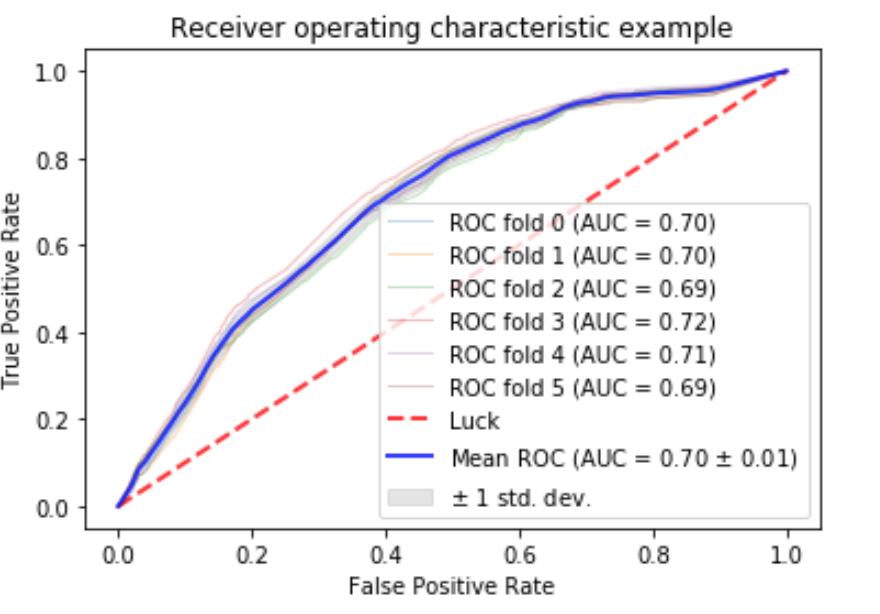
\includegraphics[width=70mm]{./images/modelperformance-baseline-roc}}
\subfigure[Precision Recall]{\label{fig:b}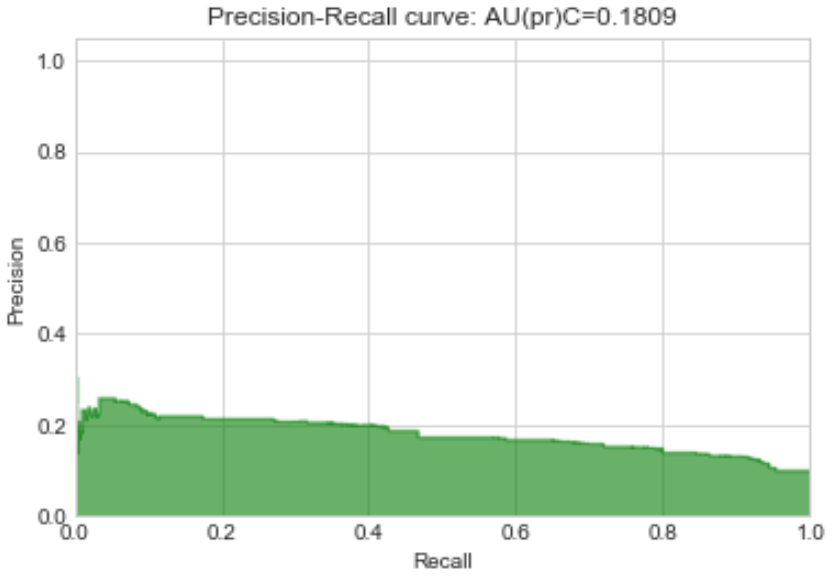
\includegraphics[width=70mm]{./images/modelperformance-baseline-pr}}
\caption{Baseline Model Performance}
\label{BaselineModelPerformance}
\end{figure}

As Figure \ref{BaselineModelPerformance} shows, even with just basic Demographic and Static Features, the model does OK. Average AUROC is about 0.70, and precision recall curve is about 0.1809 (with baseline mortality rate of about 9\% as we saw in Section \ref{Data Exploration}.

\subsubsection{Improved Model: With Structured Clinical Data}
This model will be fit and discussed by the Final Draft.

\subsubsection{Best Model: Using LDA}
This model will be fit and discussed by the Final Draft. See Table \ref{LDA} for an example of topics that were extracted by LDA.

\section{Discussion}
\label{Discussion}
It was very interesting to note that even a baseline model using just basic Demographic and Static Features already does a "decent" job at predicting mortality with an AUROC of 0.70. With additional features and using the topics extracted from LDA, we definitely expect additional improvement, Ghassemi (2014) \cite{Ghassemi} reached AUROC levels of about 0.85.
\\
\\
We also were able to apply LDA and TF-IDF to extract meaningful topics for all charts in the dataset. We verified the top few topics with a clinical geriatrician, Dr. Kumar Dharmarajan who provided meaningful clinical context to the topics abstracted. 

\section{Conclusion}
\label{Conclusion}
EHR systems contain an increasingly growing amount of data that includes unstructured data such as clinical notes. The usage of this data becomes paramount as voluminous records make manual synthesis difficult, but provide a potentially rich set of features to learn from. We hope that the work here can help diagnose a patient's condition and stratify patients into high risk, especially in an already risky environment to make clinical care more efficient.

  \begin{thebibliography}{1}
    \bibitem{Afessa} Afessa B, Keegan MT. Predicting mortality in intensive care unit survivors using a subjective scoring system. Crit Care. 2007;11(1):109.   
    \bibitem{DeSalvo} DeSalvo KB, Fan VS, McDonell MB, Fihn SD. Predicting mortality and healthcare utilization with a single question. Health Serv Res. 2005;40(4):1234-46. 
    \bibitem{Ghassemi} Ghassemi M, Naumann T, Doshi-Velez F, et al. Unfolding Physiological State: Mortality Modelling in Intensive Care Units. KDD. 2014;2014:75-84.
    \bibitem{Johnson} Johnson AEW, Mark RG. Real-time mortality prediction in the Intensive Care Unit. AMIA Annu Symp Proc. 2018;2017:994-1003. Published 2018 Apr 16.
    \bibitem{Lipshutz} Lipshutz Angela KM, Feiner John R, Grimes Barbara, Gropper Michael A. Predicting mortality in the intensive care unit: a comparison of the University Health Consortium expected probability of mortality and the Mortality Prediction Model III. Journal of Intensive Care. 2016
    \bibitem{Silva} Silva I, Moody G, Scott DJ, Celi LA, Mark RG. Predicting In-Hospital Mortality of ICU Patients: The PhysioNet/Computing in Cardiology Challenge 2012. Comput Cardiol (2010). 2012;39:245-248.
	\bibitem{Siontis} Siontis GCM, Tzoulaki I, Ioannidis JPA. Predicting Death: An Empirical Evaluation of Predictive Tools for Mortality. Arch Intern Med. 2011;171(19):1721–1726. doi:10.1001/archinternmed.2011.334
	\bibitem{Teasdale} Teasdale Graham, Stocchetti Nino, Mass Andrew, Murray Gordon. Predicting Mortality in Critically Ill Patients. Critical Care Medicine. (2015). 2015;43:471-472
  
  \end{thebibliography}
\end{document}